\chapter{Results}    \label{results}
\section{Recruitment of Rvs to endocytic sites}

	\subparagraph{Curvature sensing or generation? }
	\mbox{}\\
Cellular membrane shape is a result of properties like rigidity, tension, intracellular pressure, and are influenced by the lipid composition and the proteins embedded in it1,2. Since tension, pressure, and rigidity all oppose membrane deformation, energy is required to deform and bend it. BAR domains can generate curvature if the energy required to deform the membrane is less than the energy spent in binding flat membrane.

\vspace{5mm}
			
Scaffolding as a curvature-generation mechanism has been extended to various types of BAR proteins, (Arkhipov et al., 2009; Frost et al., 2008; Henne et al., 2007; Itoh et al., 2005; Pykalainen et al., 2011; Saarikangas et al., 2009; Shimada et al., 2007; Yu and Schulten, 2013). In order for BAR scaffolds to impose membrane curvature, some requirement have to be met3: they have to have present a large membrane-interacting surface that can mediate membrane binding, have intrinsic curvature that can be imposed on the surface, and have a rigid structure that can overcome bending resistance of the membrane. Because of their shape (Peter 2004, Gallop 2006, Weissenhorn 2005), and their capacity to oligomerize into large assemblies on tubes (Mim 2012, Mizuno 2010, Takei 1999, Yin 2009), it has been suggested that BAR domains impose their shape on the membrane, and generate membrane curvature in cells. Further, tubulation both in-vivo and of liposomes is dependent on the rigidity of the central crescent-shaped domain4. The N-helix of NBAR domains can generate curvature independently of the BAR scaffold (Varkey 2010, Westphal and Chandra 2013).

\vspace{5mm}
For endophilin, the BAR domain is relatively far from the membrane, suggesting a mechanism dependent on the N-helix (Jao 2010). Different BAR domains thus likely employ different mechanisms to interact with the membrane for generating vesicles, and tubes (Ambroso 2014). For endophilin, for example, the N-helix is necessary for liposome binding5, while that of amphiphysin is important, but not necessary6. 

\vspace{5mm}
Curved BAR proteins that can induce curvature are also able to sense curvature: in-vitro, BAR domains show a preferential-binding to vesicles based on their intrinsic curvature. Curvature-generation and sensing seem to intrinsically couple mechanisms. That BAR domains are able to generate curvature does not imply that this is their function, at least in endocytocis: in-vivo, the significance of curvature-generation is not determined. Tracking over thirty different endocytic proteins in NIH-3TC cells (derived from mouse fibroblasts), TIRF imaging shows that Endophilin2 and Amphiphysin1 arrive late in the endocytic time-line right before scission7, suggesting they arrive when membrane tubes are already formed. 

\vspace{5mm}
In the case of Rvs, centroid tracking and averaging shows that the complex similarly localizes to sites late in the endocytic timeline, close to scission8. CLEM studies have further shown that Rvs localizes to sites after the membrane invaginations are about 60nm deep into the cytoplasm: Rvs localizes once membrane curvature is established. Whether this localization is dependent on membrane curvature, recognized by the BAR domain has not been shown. 

\vspace{5mm}
Rvs localization in yeast endocytosis
As has been shown before, Rvs localizes to endocytic patches at the yeast plasma membrane in the late scission-stage. When imaged at the plasma membrane, rather than a slow inward movement typical for coat proteins like Sla1, Rvs167-GFP shows a sharp jump into the cytoplasm, concomitant with scission8,9. The average lifetime of Rvs167-GFP is about 7secs, as measured by epifluorescence microscopy at the equatorial plane of a haploid yeast cell. 


	\subsection{BAR domain senses membrane curvature in-vivo}
	Rvs167 without the BAR domain, that is, Rvs167-delsh3 localizes to cortical patches (Fig.2.3). In order to test whether this localization is because of membrane curvature, I studied its dynamics in sla2del cells. Sla2 is a coat protein that acts as a linker between the membrane and the actin cytoskeleton, and allows forces generated within the actin network to be transmitted to the membrane10. In sla2del cells, rather than cortical actin patches, actin “flames” appear inside the cytoplasm. Electron microscopy shows that the membrane is flat in these cells: although actin is able to polymerize and recruit other actin-binding proteins, actin forces are decoupled from the membrane (Fig.2.2 schematic). 
	
	\vspace{5mm}
	In sla2del cells, Rvs167-GFP is recruited to the plasma membrane (Fig.2.3), while in sla2del cells expressing Rvs167-delsh3GFP (henceforth BAR-GFP), localization is removed, except for rare transient patches at the plasma membrane. 

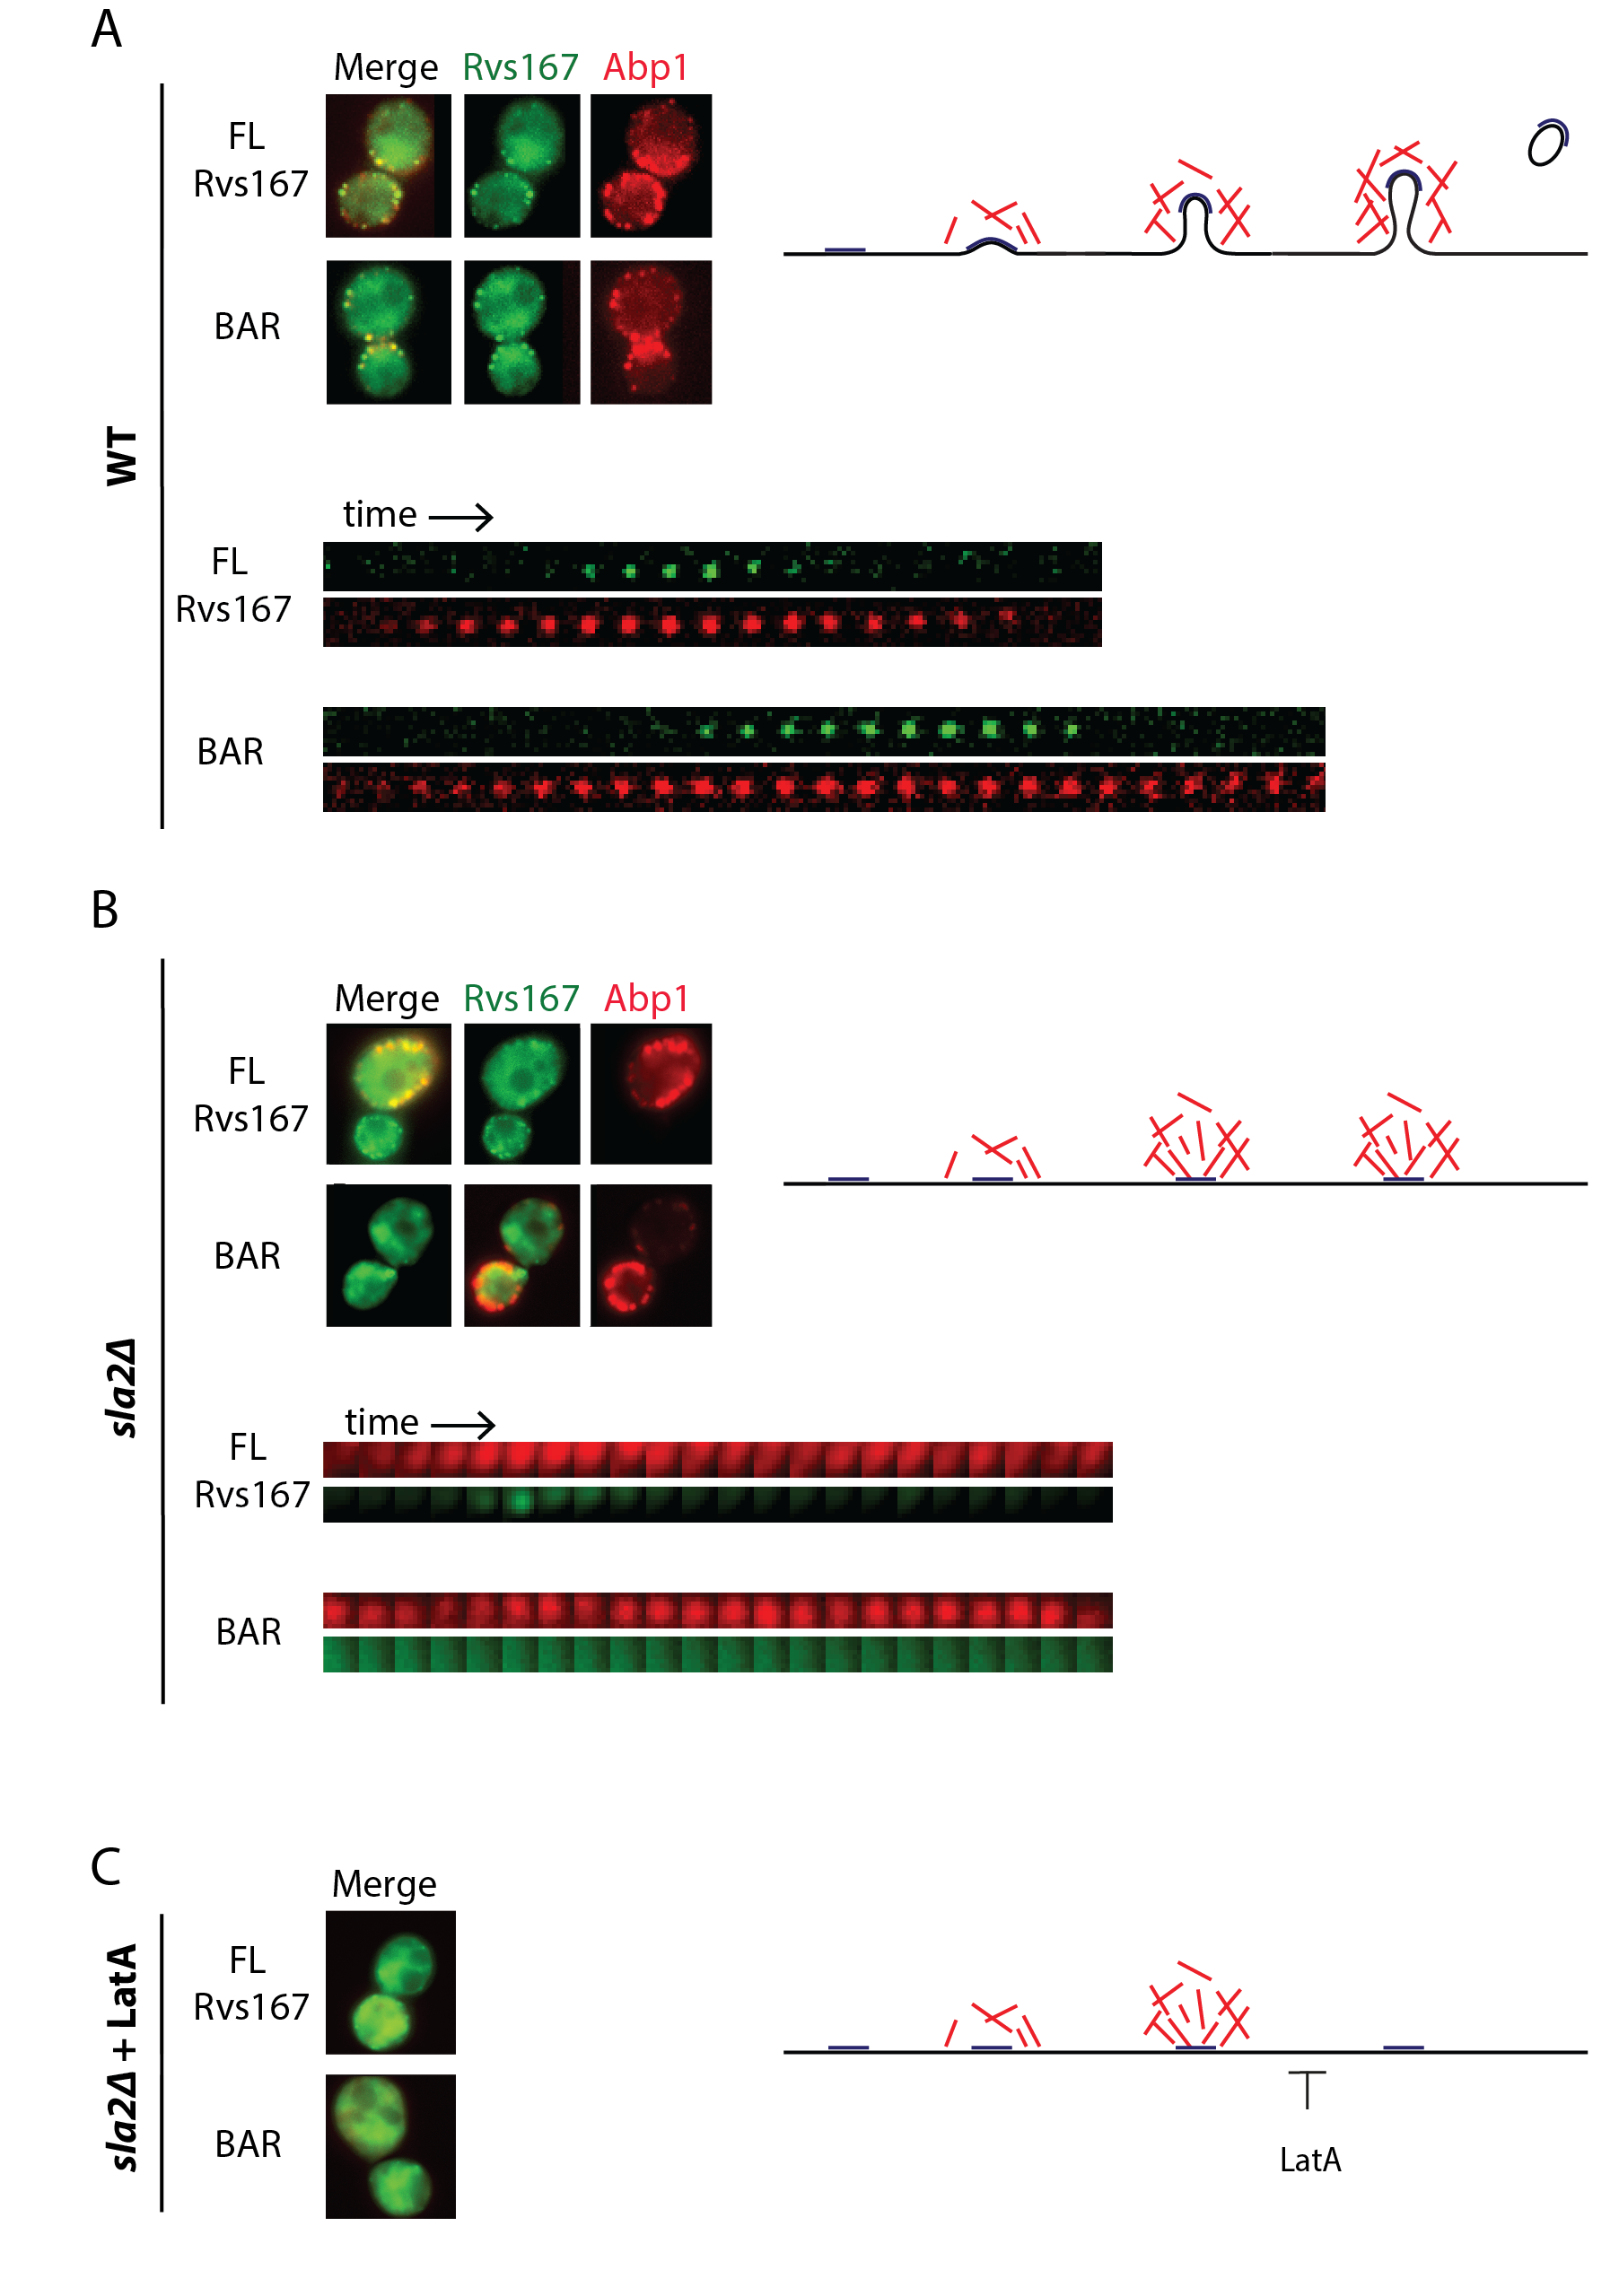
\includegraphics[width=20cm,height=20cm,keepaspectratio]{../../../figures/results_final/sla2_del_final3}
	
	\subsection{SH3 domain is able to recruit Rvs in an
		actin-independent  	\\ manner}
	Full-length Rvs is able to localize to cortical patches in Sla2del cells. This localization must come from the SH3 domain, since BAR alone does not localize in these cells. We expected that the SH3 domain must interact with WASP or actin-binding proteins: an interaction with Abp1 has been shown, as well as with Las17, type I Myosins, and Vrp1. In order to prove this, I imaged BAR-GFP in cells treated with the actin sequestering agent LatrunculinA (LatA). LatA is a sea-sponge toxin that binds monomeric actin, and prevents incorporation of actin into filaments. Since a high actin turnover is required at endocytic sites, LatA effectively disassembles WASP components and other actin-binding proteins of the endocytic machinery, and blocks endocytosis. 
	
	\vspace{5mm}
	Surprisingly, full-length Rvs is localized to the plasma membrane in spite of the LatA treatment, suggesting that the SH3 domain is able to recruit Rvs to the plasma membrane. This recruitment occurs in the absence of a BAR-membrane interaction, since BAR-GFP localization is completely removed in LatA treated cells. Rvs167-GFP patches are transient, so an assembly-diassembly mechanism is mediated by the SH3 domain outside of its BAR domain interaction. Localization of Rvs161, which does not have an SH3 domain, is also removed by LatA treatment, supporting the conclusion that the BAR domain senses membrane curvature in-vivo. 

	\subsection{What does the SH3 domain interact with?}
		\subsubsection{Vrp1}
		\subsubsection{Type 1 myosins}
		\subsubsection{Las17}


	\subsection{Other potential mechanisms of assembly/ disassembly of Rvs}		
			\subsubsection{Interaction with Calmodulin}
			\subsubsection{FBAR protein Bzz1}
				
\section{Role of the SH3 domain}	
Is likely that SH3 domains, are involved in modulating oligomerization (5, 14) and MC-S, G (15, 82). 	
\section{Role of the N-helix}			
		
\section{Scission mechanisms}

	\subsection{Membrane scission is not dependent on Vps1}
	\subsection{Yeast Synaptojanins do not influence scission timing}
	\subsection{Protein friction does not induce membrane scission }
	\subsection{Scission timing is determined by actin forces, \\
		BAR domains prevent scission}